\chapter{BACKGROUND}

We present the shared prerequisites to our articles.


\section{Deep Learning}

Deep learning is a subfield of machine learning that uses neural
networks.

Feedforward neural networks (FNNs) can be expressed as
$\vec{h}_i = f_i({\matr{W}_i}^\intercal \vec{h}_{i - 1} + \vec{b}_i)$, where
$\vec{h}_i$ is a hidden unit, $\matr{W}_i$ is the weight matrix of layer~$i$ of
the neural network, $\vec{b}_i$ is a bias vector and $f_i$ is a non-linearity
or link function, such as the sigmoid function $f(x) = 1/(1 + e^{-x})$.


\section{Convolutional Neural Networks (CNNs)}

Convolutional neural networks (CNNs) are a type of neural network designed to
model data that is arranged in a grid, as the pixels in an image are arranged.
While each neuron in a layer of an FNN is connected to all neurons in its
previous layer via a matrix multiplication, neurons in a layer of a CNN are
only locally connected to neurons in the previous layer.

We explain the meaning of ``locally connected''. We assume that a given layer
has a 3-D tensor $\tens{V}$ as input, where in addition to the single dimension
of the hidden unit vector $\vec{h}$ of FNNs, there are two extra spatial
dimensions (e.g. $x$ and $y$ dimensions of an image).  A CNN connects the input
tensor $\tens{V}$ to an output tensor $\tens{Z}$ through a 4-D tensor
$\tens{K}$ called a ``kernel'', which contains the CNN's learned parameters.

The kernel has one dimension matching the ``channels'' (the third, i.e.\
non-spatial, dimension of the input tensor $\tens{V}$), one dimension that
becomes the channels of the output tensor $\tens{Z}$, and two spatial
dimensions that are normally much smaller than the input feature tensor
$\tens{Z}$'s spatial dimensions. E.g.\ for an input image of dimensions $224
\times 224$ pixels and~\num{3} colour channels, a CNN kernel's spatial
dimensions would normally be $3 \times 3$. The CNN kernel's weights are thus
shared spatially, and each element of the output tensor is contributed to only
by a $3 \times 3$ spatial region of the input tensor, via a sum over
channel-wise matrix multiplications of the kernel strictly over that spatial
region.

Formally, each element $\tens{Z}_{i, j, k}$ of the output tensor corresponds to the
sum given in Equation~\ref{eqn:convolution}, where~$i$ is the index of the
output channel and $j$ and $k$ are the spatial indices of the output element.
The index~$l$ runs over the input channels, while~$m$ and $n$ are restricted by
the spatial dimensions of the kernel, e.g.\ in our $3 \times 3$ kernel example
we have $m, n \in \{-1, 0, 1\}$.

\begin{equation}
        \tens{Z}_{i, j, k} = \sum_{l, m, n} \tens{V}_{l, j + m, k + n} \tens{K}_{i, l, m, n}
\label{eqn:convolution}
\end{equation}

\begin{figure}
\centering
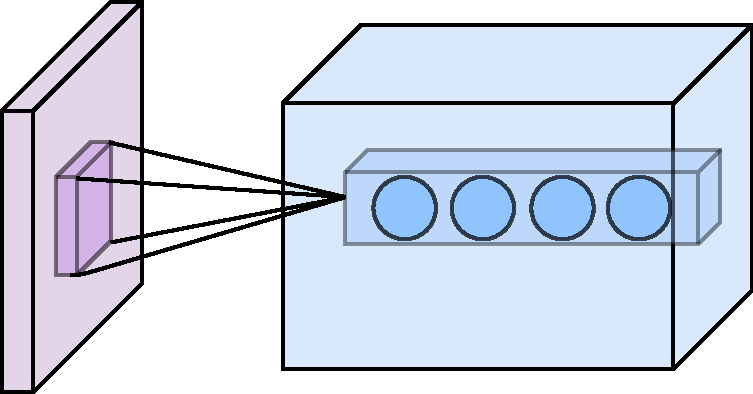
\includegraphics[width=0.8\textwidth]{Figures/cnn.pdf}
\caption{Two subsequent layers of a convolutional neural network.}
\label{fig:cnn}
\end{figure}

Figure~\ref{fig:cnn} depicts the interaction between two subsequent layers of a
CNN\@. The kernel~$\tens{K}$ (inner box on the left) is multiplied with a
volume of the input~$\tens{V}$ (outer box on the left) to produce a single unit
consisting of a column of values at a single spatial location in the
output~$\tens{Z}$.

CNNs generalize well in comparison to FNNs on visual data, since the number of
parameters are dramatically reduced compared with an equivalent FNN by sharing
parameters in the spatial dimensions~\cite{lecun-89}. This is an example of
improving generalization of neural networks by using prior knowledge (i.e.\ in
this case, the spatial invariance of image data) when constructing a model for
a given type of data.

In the case of the visual question-answering task, we make use of a particular
CNN architecture called a ResNet~\cite{he2016deep} that has~\num{152} layers.
This CNN architecture has been pre-trained on a large dataset of image data to
extract useful generic feature representations from images.
The fusion operator takes this image feature representation as input, along
with a feature representation of the question, in order to predict an answer to
the posed question conditioned on the image.


\section{Recurrent Neural Networks (RNNs)}

Like CNNs, Recurrent Neural Networks~(RNNs)~\cite{rumelhart1986learning} are a
type of neural network model that has been invented using prior knowledge of
the type of data distribution relevant to the given task.
In particular, RNNs are designed to work on sequential data of arbitrary
length, such as time-series data including stock prices over time, or language
data, where the inputs are the word or character tokens making up sentences and
paragraphs.

Instead of sharing parameters spatially as in CNNs, RNNs share parameters over
time. The output at each timestep~$t$, $\vect{a}{t}$, takes as input both the
``hidden state'' from the previous timestep~$\vect{h}{t - 1}$ as well as the
input~$\vect{x}{t}$ of the current timestep, as given by
Equation~\ref{eqn:vanilla-rnn}.

\begin{equation}
        \vect{a}{t} = \matr{W}\vect{h}{t - 1} + \matr{U}\vect{x}{t} + \vec{b}
\label{eqn:vanilla-rnn}
\end{equation}

The hidden state~$\vect{h}{t}$ is related to the output~$\vect{a}{t}$ of a
given timestep~$t$ by the link function $f$, i.e.\
$\vect{h}{t} = f(\vect{a}{t})$, where $f$ is usually~$\tanh$.


\section{Skip-Thought Vectors}

Skip-thought vectors~\cite{kiros2015skip} is a method of encoding a feature
representation from a sentence, in such a way that the feature representation
can be re-used as a generic, continuous sentence representation in a variety of
tasks.
In skip-thought vectors, an ``encoder'' RNN is trained to extract a feature
representation with enough context from the current sentence in order to
predict words in the sentences immediately preceding and following the current
sentence.

As their basic neural network component, skip-thought vectors use a type of RNN
called a Gated Recurrent Unit (GRU)~\cite{cho2014ontheproperties}.
The GRU is similar to the vanilla RNN given by Equation~\ref{eqn:vanilla-rnn},
except that there are extra outputs $\vect{r}{t}$ and $\vect{z}{t}$ (and
corresponding weight matrices $\matr{W}_r$, $\matr{U}_r$ and $\matr{W}_z$,
$\matr{U}_z$) that are used to ``turn on or off'' both the contribution of the
hidden state~$\vect{h}{t - 1}$ in Equation~\ref{eqn:vanilla-rnn}, and to
control the update of the hidden state from timestep~$t - 1$ to $t$, as given
by Equation~\ref{eqn:gru-update}.

\begin{equation}
        \vect{h}{t} = (1 - \vect{z}{t}) \odot \vect{h}{t - 1} + \vect{z}{t} \odot \vect{\widetilde{h}}{t}
\label{eqn:gru-update}
\end{equation}

In Equation~\ref{eqn:gru-update},
$\vect{z}{t} = \sigma(\matr{U}_z\vect{h}{t - 1} + \matr{W}_z\vect{x}{t})$,
where $\sigma(\cdot)$ is the sigmoid function. So,
Equation~\ref{eqn:gru-update} is a linear interpolation controlled by the
``update gate'' $\vect{z}{t}$ between the previous hidden state
$\vect{h}{t - 1}$ and the would-be current
hidden-state~$\vect{\widetilde{h}}{t}$.

Regardless of the specific details of GRUs, the relevance to this paper is that
skip-thought vectors use an RNN as an encoder, which encodes the sequence
of words in a sentence into a feature representation corresponding to that
sentence, where the feature representation is a vector of real-valued numbers.

In this work, skip-thought vectors are used to extract a feature representation
from the question, which is coupled with the feature representation extracted
from the image as a dual input to a multi-modal fusion operator, which takes
the two feature-representation inputs and produces an output prediction as to
the answer to the given question, conditioned on the image.


\section{Attention}

Attention in deep learning is an operator motivated by the idea that making
predictions for a given task may require weighing a subset of inputs more
heavily than others, or even focusing on a single subset of inputs exclusive of
all others.
In vision, attention is motivated by the human fovea, which is responsible for
our sharp central vision used for demanding vision tasks such as driving and
reading.
In natural language, we structure our sentences differently depending on which
cues in our environment capture our focus~\cite{myachykov2005attention}.

The deep learning community drew inspiration from the importance of attention
in human perception, with early work using Boltzmann machines to combine foveal
glimpses~\cite{larochelle2010learning}, and using foveated images for
recognition and tracking~\cite{denil2012learning}.
Graves used differentiable attention in the form of weights of a mixture of
Gaussians over shifts for handwriting synthesis~\cite{graves2013generating}.
Mnih et al.\ used non-differentiable attention trained with reinforcement
learning to perform classification with reduced computation by observing only
predicted regions of an image~\cite{mnih2014recurrent}.
Bahdanau et al.\ introduced attention models for neural machine translation,
by predicting a set of weights~$(\alpha_1, \dots, \alpha_t)$ over the sequence
of hidden state vectors~$(h_1, \dots, h_t)$ over~$t$ timesteps output by an
encoder-decoder architecture~\cite{cho2014ontheproperties}.

In the following we describe mathematically the attention operator relevant to
this thesis.
We first introduce attention on sequences, i.e., 1D attention, before
describing our generalization to spatial and spatiotemporal domains.


\subsection{Scaled Dot-Product Attention}

Suppose we are given two matrices~$Q$ and~$K$ in~$\mathbb{R}^{t_1 \times c}$
and~$\mathbb{R}^{t_2\times c}$, respectively, representing input
sequences~$Q \equiv (q_1, \dots, k_{t_1})$ and~$K \equiv (k_1, \dots, k_{t_2})$
of~$t_i$ vectors~$q_t$ and~$k_t$, for example sequences of word embeddings.
We wish to compute an output sequence~$Y \equiv (y_1, \dots, y_{t_1})$ that is
a linear combination of a third sequence~$V \equiv (v_1, \dots, v_{t_2})$ whose
weights in the linear combination depend on the affinity between pairs of
vectors in~$Q$ and~$K$.

In their work introducing Transformers for NLP tasks, Vaswani et
al.~\cite{vaswani2017attention} interpreted attention in the framework of data
retrieval, and we follow their perspective here.
An attention layer retrieves vector elements of the value~$V$ based on the
similarity of a query vector element from~$Q$ with the key vector from~$K$ that
corresponds to the value.
From our perspective, attention is a method for using query~$Q$ to perform a
lookup in the values~$V$, indexed by the key~$K$.

In particular, output vectors~$y_t \in \mathbb{R}^c$ are a linear combination
of all value vectors~$v_i$, with the weighting of~$v_i$ in the linear
combination dependent on the similarity of query vector~$q_t$ with key
vector~$k_i$.
At this point in our definition of attention we are faced with a decision about
how we should quantify the similarity between query vector~$q_t$ and key
vector~$k_i$.
Vaswani et al. refer to the similarity between query and key as attention's
``compatibility function''.
One possible compatibility function would be the ``additive alignment model''
used by Bahdanau et al.~\cite{bahdanau2015neuralmt}, which computes
compatibility by concatenating query and key and using this concatenated vector
as input to a feedforward neural network.
Another possibility is to use a dot-product compatibility function, which
computes the compatibility between query and key as their dot product.

The dot-product compatibility function has similar theoretical complexity to
additive compatibility, but has the advantage of being able to compute all
pairwise query-key compatibilities in a single matrix
multiplication~$QK^\intercal$.
Matrix multiplication is highly optimized on modern compute hardware, and
therefore dot-product attention runs faster than additive attention out of the
box.
For this reason, we use dot product attention in our work.

Our overall attention function is therefore

\begin{equation}
\mathtt{Attention}\big(Q, K, V\big) = \softmax{}\left(\frac{QK^\intercal}{\sqrt{c}}\right) V.
\label{eqn:background:attndefn}
\end{equation}

In Equation~\ref{eqn:background:attndefn} we scale by the squareroot of the
dimension of query and key vectors~$\sqrt{c}$ in the argument to softmax.
The intuition behind this scaled dot product attention, as given by Vaswani et
al., is that if scalar elements of query and key vector were drawn from
independent zero-mean, unit-variance distributions, then the magnitude of the
query-key dot product grows like the squareroot of their dimension.
Therefore for query-key combinations whose dimensions are large, without
scaling it is likely that the softmax would saturate early in training, causing
vanishing gradients.


\subsection{Multi-Head Attention}

Building on scaled dot-product attention, multi-head attention is another
technique to improve the capacity while reducing the computation of attention.
Multi-head attention breaks the attention computation up into multiple
attention computations determined by the ``number of attention heads''
hyperparameter~$n_h$.
We illustrate multi-head in Figure~\ref{fig:background:multiheadattn}.

\begin{figure}
\centering
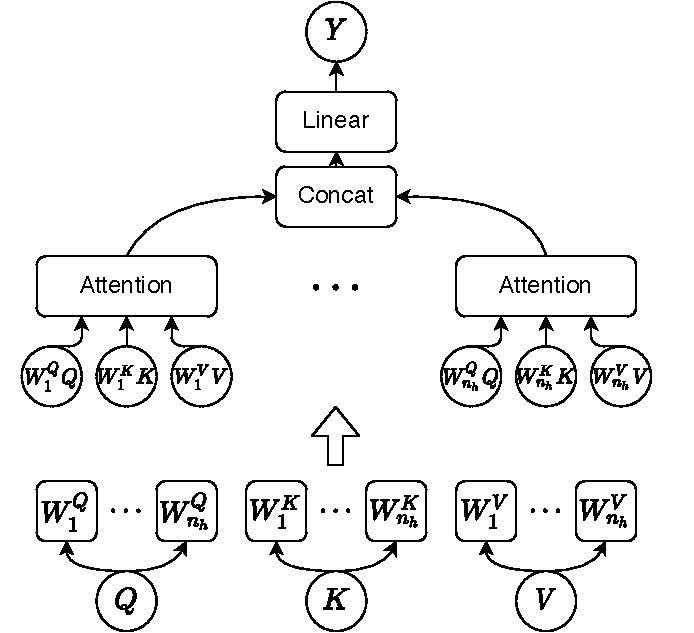
\includegraphics[width=0.8\textwidth]{Figures/multihead-attention.pdf}
\caption{Multi-head attention.
         Adapted from Vaswani et al.~\cite{vaswani2017attention}.}
\label{fig:background:multiheadattn}
\end{figure}

A single attention operator as given by Equation~\ref{eqn:background:attndefn}
would have a theoretical complexity proportional to the query and key
dimension~$c$.
In multi-head attention, we project query, key and value vectors by learned
weights~$W^Q_i \in \mathbb{R}^{c\times c/n_h}$,
$W^K_i \in \mathbb{R}^{c\times c/n_h}$,
and~$W^V_i \in \mathbb{R}^{c\times c/n_h}$, respectively, where~$i$
ranges from~$1$ to~$n_h$.
We then perform the~$n_h$ attention operations on the projected query, key and
value vectors.
Hence, multi-head attention on the projected vectors has the same theoretical
complexity as a single attention operator on the original query, key and value
vectors.
Intuitively, multi-head attention has the advantage that each~$i$th head can
specialize in learning to attend to particular features corresponding to the
affine subspace spanned by columns of the~$i$th projection weight matrix.

We concatenate outputs of the multi-head attention layers and feed the
resulting~$c$-vector into an output linear layer to produce the output~$Y$.
This final concatenation and projection step aggregates information from the
multiple attention heads, for example to combine information gathered by
different attention heads ``looking at'' different regions of an image.


\subsection{Positional Encoding}

Up until this point in our description of attention, our attention operators
are unable to incorporate positional information, since query and key vectors
interact pairwise with each other.
Whlie recurrent networks have a positional inductive bias, both convolutional
and attention networks are translation equivariant and require injection of
position information to perform position-dependent tasks such as
sequence-to-sequence learning.
Following Gehring et al.'s use of positional encodings for convolutional
sequence-to-sequence networks~\cite{gehring2017convolutional}, in Transformers
Vaswani et al.~\cite{vaswani2017attention} introduced positional encodings to
attention.

Positional encoding means adding to each key vector another vector with encoded
positional information.
Therefore with positional encoding Equation~\ref{eqn:background:attndefn} becomes

\begin{equation}
\mathtt{Attention}_E\big(Q, K, V\big) = \softmax{}\left(\frac{Q(K + E)^\intercal}{\sqrt{c}}\right) V,
\label{eqn:background:posenc-attn}
\end{equation}

where positional encoding matrix~$E \in \mathbb{R}^{t_2\times c}$ contains a
unique positional encoding~$c$-vector for each of the~$t_2$ elements in our
queried sequence.

We consider positional encodings made up of learned embeddings, and sinusoidal
positional encodings.
In the case of learned embeddings, the positional encoding matrix~$E$ is
initialized at the beginning of training and updated along with the rest of the
model parameters using backpropagation.
Sinusoidal positional encodings, on the other hand, are not learned and instead
are fixed to a vector of values from a set of sinusoids of varying period
evaluated at the timestep, or sequence element,~$t$.
In particular,

\begin{equation}
\begin{split}
E_{t, 2i} &= \sin\left(\frac{t}{\tau^{2i/c}}\right) \\
E_{t, 2i + 1} &= \cos\left(\frac{t}{\tau^{2i/c}}\right)
\end{split}
\end{equation}

where~$\tau$ is a fixed constant, for example Vaswani et al. fixed~$\tau$
to~\num{10000}.

% \subsection{Sparse Attention}


% \subsection{Transformers}


\section{Fusion}

We refer to a topic specific to multimodal applications as fusion.
Following Lahat et al.'s definition~\cite{Lahat2015MultimodalDF}, multimodal
applications involve observing a single phenomenon using data collected from
multiple distinct sensors.
We refer to the raw stream of data collected from each sensor as a modality.
For example, we could treat a video as a multimodal application by making use
of RGB video frames, extracted optical flow and audio as input.
Autonomous driving also makes use of multimodal fusion to combine information
collected from multiple sensors, including LiDAR, radar, and camera
sensors~\cite{Feng2019DeepMO}.

Multimodal fusion refers to the technique by which information extracted from
these multiple raw data streams is combined.
Using fusion holds the promise of producing superior predictions by leveraging
the complementary information contained in separate data streams.
As an example proposed by Kazakos et al.~\cite{kazakos2019TBN}, consider an
egocentric action recognition system that is given as input a video of a person
at a kitchen sink.
When the sink tap is occluded, the audio signal provides a discriminative cue
for the actions ``turn tap on'' and ``turn tap off''.
On the other hand, video input would be more useful for predicting ``wiping
hands'', which has no discriminative auditory signal.
Hence, in this case multiple sensors provide the multimodal action recognition
system with complementary inputs leading to superior predictions.

We can categorize multimodal fusion architectures into early and late fusion.

Fusion operators themselves have varying designs.
